\documentclass[border=4pt,12pt]{standalone}
% House style for redrawn exam diagrams (diagram-v4: 0.4pt lines, filled -latex arrows, fine dashes; stipple and hatching drawn as real dots/lines (no PDF/SVG patterns, so they render in every browser and at any scale); transparent background). Every figure \input's this.
\usepackage{amsmath,amssymb}
\usepackage{txfonts}
\usepackage{pdfrender,xcolor}
% \halo{text}: label on shading. The shading stops just around each letter's outline (a thin knock-out that follows the
% glyphs, like the papers' typesetting), never a box. Owner: "I don't want a box around the text".
\newcommand{\halo}[1]{\leavevmode\rlap{\pdfrender{TextRenderingMode=2,LineWidth=2.2pt,LineJoinStyle=1,StrokeColor=white,FillColor=white}#1}#1}
\usepackage{tikz,pgfplots}
\pgfplotsset{compat=1.18}
\usetikzlibrary{arrows.meta,calc,angles,quotes,patterns,patterns.meta,intersections,positioning,decorations.markings,shapes.geometric}
% Stipple and hatching are drawn as actual dots / lines clipped to the region (path picture), NOT as pattern fills:
% SVG <pattern> fills vanish or blur when browsers scale the image, so the owner could not see the shading.
% Each dot is a 0.72pt square (keeps SVGs small; reads as a dot at print size). Dots sit on one global staggered grid, so neighbouring regions line up.
\makeatletter
\newdimen\ex@x \newdimen\ex@y \newdimen\ex@xa \newdimen\ex@ya \newdimen\ex@xb \newdimen\ex@yb \newcount\ex@row
\def\exam@stipplecolor{black!75}\def\exam@dotr{0.42pt}\def\exam@dotgap{2.5}
\def\ex@rowdots{\ifdim\ex@x<\ex@xb \pgfpathrectangle{\pgfqpoint{\dimexpr\ex@x-0.36pt\relax}{\dimexpr\ex@y-0.36pt\relax}}{\pgfqpoint{0.72pt}{0.72pt}}\advance\ex@x by \exam@dotgap pt\relax\expandafter\ex@rowdots\fi}
\def\exam@stipple{%
  \pgftransformreset% dots are sized in real points even inside scaled pictures
  \pgfpointanchor{path picture bounding box}{south west}\ex@xa=\pgf@x \ex@ya=\pgf@y
  \pgfpointanchor{path picture bounding box}{north east}\ex@xb=\pgf@x \ex@yb=\pgf@y
  \pgfsetfillcolor{\exam@stipplecolor}\pgfmathsetmacro\ex@h{\exam@dotgap/2}%
  \pgfmathtruncatemacro\ex@r{floor(\ex@ya/\ex@h)-1}\ex@row=\ex@r\relax
  \ex@y=\ex@r\dimexpr\ex@h pt\relax
  \loop\ifdim\ex@y<\ex@yb
    \pgfmathtruncatemacro\ex@c{floor(\ex@xa/\exam@dotgap)-1}\ex@x=\ex@c\dimexpr\exam@dotgap pt\relax
    \ifodd\ex@row \advance\ex@x by \ex@h pt\fi
    \ex@rowdots
    \advance\ex@y by \ex@h pt \advance\ex@row by 1
    \ifnum\numexpr\ex@row-(\ex@row/4)*4\relax=0 \pgfusepath{fill}\fi% flush every 4 rows: bounded TeX memory, few clip copies in the SVG
  \repeat\pgfusepath{fill}}
\newdimen\ex@d
\def\exam@hatch#1{% #1 = 1 for /, -1 for \ ; lines 45 degrees, 3pt apart
  \pgftransformreset
  \pgfpointanchor{path picture bounding box}{south west}\ex@xa=\pgf@x \ex@ya=\pgf@y
  \pgfpointanchor{path picture bounding box}{north east}\ex@xb=\pgf@x \ex@yb=\pgf@y
  \ex@d=\dimexpr\ex@yb-\ex@ya\relax \ex@x=\dimexpr\ex@xa-\ex@d\relax
  \loop\ifdim\ex@x<\ex@xb
    \ifnum#1>0 \pgfpathmoveto{\pgfqpoint{\ex@x}{\ex@ya}}\pgfpathlineto{\pgfqpoint{\dimexpr\ex@x+\ex@d\relax}{\ex@yb}}%
    \else \pgfpathmoveto{\pgfqpoint{\ex@x}{\ex@yb}}\pgfpathlineto{\pgfqpoint{\dimexpr\ex@x+\ex@d\relax}{\ex@ya}}\fi
    \advance\ex@x by 4.24pt
  \repeat
  \pgfsetlinewidth{0.4pt}\pgfsetstrokecolor{black}\pgfusepath{stroke}}
\def\examstipple{\exam@stipple}\def\examhatch{\exam@hatch}\def\examsetstipplecolor#1{\def\exam@stipplecolor{#1}}\def\examsetdotgap#1{\def\exam@dotgap{#1}}
\makeatother
% (legacy pattern kept for old files)
% staggered stipple like the NESA papers' dotted shading
\pgfdeclarepatternformonly{exam stipple}{\pgfpointorigin}{\pgfqpoint{2.2pt}{2.2pt}}{\pgfqpoint{2.2pt}{2.2pt}}{%
  \pgfpathcircle{\pgfqpoint{0.55pt}{0.55pt}}{0.42pt}\pgfpathcircle{\pgfqpoint{1.65pt}{1.65pt}}{0.42pt}\pgfusepath{fill}}
\tikzset{
  every picture/.style={line width=0.6pt, >={Latex[length=2mm,width=1.3mm]}},
  curve/.style={line width=0.6pt},
  open arrow/.style={-{Latex[length=2mm,width=1.3mm]}},  % owner: filled -latex heads everywhere, no open chevrons
  aux/.style={dash pattern=on 2pt off 1.5pt, line width=0.6pt},
  shade/.code={\def\exA{#1}\def\exB{none}\ifx\exA\exB\else\pgfkeysalso{fill=black!18}\fi},
  shade/.default=on,
  shade dots/.style={fill=none, path picture={\examstipple}},
  stipple color/.code={\examsetstipplecolor{#1}},
  stipple gap/.code={\examsetdotgap{#1}},
  shade dense dots/.style={fill=none, stipple gap=1.6, path picture={\examstipple}},
  shade hatch/.style={fill=none, path picture={\examhatch{1}}},
  shade hatch reverse/.style={fill=none, path picture={\examhatch{-1}}},
  shade solid/.style={fill=black},
  pt/.style={circle, fill, inner sep=1.1pt},
  open pt/.style={circle, draw, fill=white, inner sep=1.1pt},
}
\pgfplotsset{
  exam axes/.style={axis lines=middle, axis line style={->}, xlabel={$x$}, ylabel={$y$},
    xlabel style={anchor=west}, ylabel style={anchor=south}, tick label style={font=\small},
    every axis plot/.append style={line width=0.6pt, black}, samples=200, clip=false,
    enlargelimits=false, axis on top},
}

\begin{document}
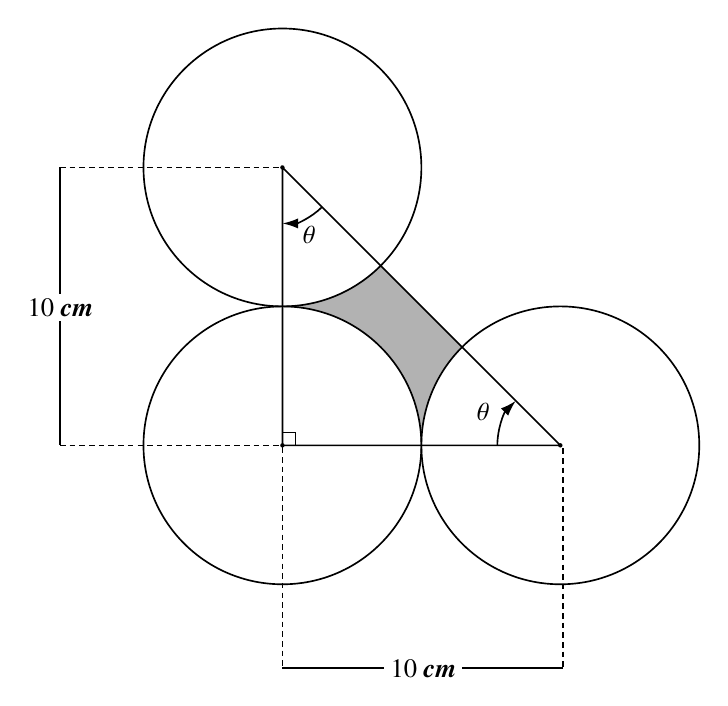
\begin{tikzpicture}[x=0.0127cm,y=-0.0127cm,font=\fontsize{9.6}{11.5}\selectfont]
\fill[black!30] (277.0,294.0) -- (279.8,294.0) -- (282.6,293.9) -- (285.4,293.7) -- (288.2,293.5) -- (291.0,293.3) -- (293.8,293.0) -- (296.5,292.6) -- (299.3,292.2) -- (302.1,291.7) -- (304.8,291.2) -- (307.5,290.6) -- (310.3,290.0) -- (313.0,289.3) -- (315.7,288.5) -- (318.4,287.7) -- (321.0,286.8) -- (323.7,285.9) -- (326.3,285.0) -- (328.9,283.9) -- (331.5,282.9) -- (334.0,281.8) -- (336.6,280.6) -- (339.1,279.4) -- (341.6,278.1) -- (344.1,276.8) -- (346.5,275.4) -- (348.9,274.0) -- (351.3,272.5) -- (353.6,271.0) -- (356.0,269.4) -- (358.2,267.8) -- (360.5,266.1) -- (362.7,264.4) -- (364.9,262.7) -- (367.1,260.9) -- (369.2,259.0) -- (371.3,257.2) -- (373.3,255.2) -- (375.3,253.3) -- (456.7,334.7) -- (454.8,336.7) -- (452.8,338.7) -- (451.0,340.8) -- (449.1,342.9) -- (447.3,345.1) -- (445.6,347.3) -- (443.9,349.5) -- (442.2,351.8) -- (440.6,354.0) -- (439.0,356.4) -- (437.5,358.7) -- (436.0,361.1) -- (434.6,363.5) -- (433.2,365.9) -- (431.9,368.4) -- (430.6,370.9) -- (429.4,373.4) -- (428.2,376.0) -- (427.1,378.5) -- (426.1,381.1) -- (425.0,383.7) -- (424.1,386.3) -- (423.2,389.0) -- (422.3,391.6) -- (421.5,394.3) -- (420.7,397.0) -- (420.0,399.7) -- (419.4,402.5) -- (418.8,405.2) -- (418.3,407.9) -- (417.8,410.7) -- (417.4,413.5) -- (417.0,416.2) -- (416.7,419.0) -- (416.5,421.8) -- (416.3,424.6) -- (416.1,427.4) -- (416.0,430.2) -- (416.0,433.0) -- (416.0,433.0) -- (415.9,427.4) -- (415.5,421.8) -- (415.0,416.2) -- (414.2,410.7) -- (413.2,405.2) -- (412.0,399.7) -- (410.5,394.3) -- (408.8,389.0) -- (407.0,383.7) -- (404.9,378.5) -- (402.6,373.4) -- (400.1,368.4) -- (397.4,363.5) -- (394.5,358.7) -- (391.4,354.0) -- (388.1,349.5) -- (384.7,345.1) -- (381.0,340.8) -- (377.2,336.7) -- (373.3,332.8) -- (369.2,329.0) -- (364.9,325.3) -- (360.5,321.9) -- (356.0,318.6) -- (351.3,315.5) -- (346.5,312.6) -- (341.6,309.9) -- (336.6,307.4) -- (331.5,305.1) -- (326.3,303.0) -- (321.0,301.2) -- (315.7,299.5) -- (310.3,298.0) -- (304.8,296.8) -- (299.3,295.8) -- (293.8,295.0) -- (288.2,294.5) -- (282.6,294.1) -- (277.0,294.0) -- cycle;
\draw (277,155) circle[radius=139];
\draw (277,433) circle[radius=139];
\draw (555,433) circle[radius=139];
\draw (277,155) -- (277,433) -- (555,433) -- cycle;
\draw (277,420) -- (290,420) -- (290,433);
\foreach \p in {(277,155),(277,433),(555,433)} \fill \p circle[radius=2.2];
\draw[->] (277,155) ++(45:56) arc[start angle=45,end angle=90,radius=56];
\draw[->] (555,433) ++(180:63) arc[start angle=180,end angle=225,radius=63];
\node at (303.5,223) {$\theta$};
\node at (477.5,400) {$\theta$};
% dimension lines
\draw[aux] (54.5,155) -- (275,155);
\draw[aux] (54.5,433) -- (275,433);
\draw (54.5,155) -- (54.5,282);
\draw (54.5,309) -- (54.5,433);
\node[anchor=base,inner sep=0] at (55,304) {10 \textbf{\textit{cm}}};
\draw[aux] (277,435) -- (277,655.5);
\draw[aux] (557.5,436) -- (557.5,655.5);
\draw (277,655.5) -- (379,655.5);
\draw (457,655.5) -- (557.5,655.5);
\node[anchor=base,inner sep=0] at (418,665) {10 \textbf{\textit{cm}}};
\end{tikzpicture}
\end{document}
